\documentclass[11pt]{beamer}
\usetheme{Madrid}
\usefonttheme{serif}

\usepackage[utf8]{inputenc}
\usepackage[spanish]{babel}
\usepackage[T1]{fontenc}

\usepackage{tikz}
\usetikzlibrary{positioning}
\usepackage{amsmath}
\usepackage{amsfonts}
\usepackage{amssymb}
\usepackage{multicol,pst-plot}
\usepackage{graphicx}
\graphicspath{{img/}}
\usepackage{capt-of}
\usepackage{tabularx}
\usepackage{xcolor}
\usepackage{float}
\newcolumntype{Z}{>{\Centering}X}
\newcommand{\Centering}{\centering\arraybackslash}

\DeclareMathOperator{\sen}{sen}
\DeclareMathOperator{\tg}{tg}

\setbeamertemplate{caption}[numbered]

\author[De Dios, Orjuela \& Sanchez]{Samuel De Dios \and Juan Daniel Orjuela \and David Sanchez}
\title{Teoría de Ramsey}
\newcommand{\email}{email}
\setbeamertemplate{navigation symbols}{}
\institute[]{
    Universidad del Rosario \\
    Escuela de Ciencias e Ingeniería \\
    Proyecto final de Teoría de Números \\[4pt]
    \textit{Docente:} Juan Camilo Arias
}
\date{\today}

\bibliographystyle{apalike}

% ---------------------------------------------------------

\begin{document}

\begin{frame}
    \titlepage
\end{frame}

\begin{frame}{Contenido}
    \tableofcontents
\end{frame}

% 1. Introducción (5 min)
\section{Introducción a la Teoría de Ramsey}
% DIAPOSITIVA 1: Contexto Histórico y Filosofía
\begin{frame}{Contexto Histórico y Filosofía}

    \begin{columns}

        \begin{column}{0.65\textwidth}

            \textbf{Frank Plumpton Ramsey (1903--1930)} fue un genio
            británico cuyas ideas sentaron las bases de esta rama de
            la matemática.

            \vspace{0.4cm}

            \begin{exampleblock}{Principio de Motzkin}
                \centering
                \textit{``El desorden completo es imposible''.}
            \end{exampleblock}

            \vspace{0.3cm}

            \begin{block}{Concepto Clave}
                Si un sistema es lo suficientemente grande, por más
                caótico que parezca, \textbf{siempre aparecerán
                patrones} o subconjuntos con propiedades específicas.
            \end{block}

        \end{column}

        \begin{column}{0.35\textwidth}
            % Puedes insertar aquí una imagen de Ramsey, p.ej.:
            % \includegraphics[width=\linewidth]{ramsey.jpg}
        \end{column}

    \end{columns}

\end{frame}


% DIAPOSITIVA 2: Definición Formal en Teoría de Grafos
\begin{frame}{Definición Formal}

    \begin{alertblock}{Número de Ramsey $R(r,s)$}
        Para cualquier par de enteros positivos $(r,s)$, existe un
        número mínimo $R(r,s)$ tal que, si $n \geq R(r,s)$ y se
        colorean las aristas de un grafo completo $K_n$ con
        \textbf{dos colores}, entonces necesariamente aparece:
        \begin{itemize}
            \item un subgrafo $K_r$ con todas las aristas del
                  \textbf{primer color}, o
            \item un subgrafo $K_s$ con todas las aristas del
                  \textbf{segundo color}.
        \end{itemize}
    \end{alertblock}

    \pause

    \begin{center}
        \textbf{Valores conocidos:} \quad
        $R(3,3)=6$ \quad $R(3,4)=9$ \quad $R(3,5)=14$ \quad
        $R(4,4)=18$
    \end{center}

\end{frame}


% DIAPOSITIVA 3: Los Tres Pilares y Conclusión
\begin{frame}{Método de Deducción: Los Tres Pilares}

    Para demostrar o entender un problema de Ramsey se consideran:

    \begin{enumerate}

        \item \textbf{Estructura:} Se trabaja con un conjunto grande
              (un ``universo'' de elementos).

        \item \textbf{Partición (Conteo):} Los elementos se dividen
              en categorías —colores, grupos, clases.

        \item \textbf{Inevitabilidad (Orden):} Al alcanzar un tamaño
              crítico, la densidad fuerza la aparición de un
              \textbf{patrón uniforme}.

    \end{enumerate}

    \pause
    \vspace{0.3cm}

    \begin{block}{Conclusión}
        La Teoría de Ramsey muestra que \textbf{el azar tiene
        límites}. No importa cuánto se mezclen los elementos; si el
        sistema crece lo suficiente, los patrones aparecen por
        \textit{pura necesidad matemática}.
    \end{block}

\end{frame}

% 2. Problema de la amistad (3 min)
\section{El problema de la amistad}

\begin{frame}{El problema de la amistad}
\begin{columns}
\column{0.52\textwidth}
    \begin{block}{Problema}
        En un grupo de 6 personas, ¿siempre existen 3 que se conocen mutuamente o 3 que son mutuamente desconocidos?
    \end{block}
    Modelamos como el grafo completo $K_6$:
    \begin{itemize}
        \item Aristas \textcolor{red}{rojas}: se conocen
        \item Aristas \textcolor{blue}{azules}: desconocidos
    \end{itemize}
    \begin{alertblock}{Pregunta}
        ¿Toda 2-coloración de $K_6$ tiene un triángulo monocromático?
    \end{alertblock}
\column{0.45\textwidth}
\begin{center}
\begin{tikzpicture}[scale=1.0]
    \foreach \i/\ang in {0/90,1/30,2/-30,3/-90,4/-150,5/150} {
        \coordinate (v\i) at (\ang:1.4cm);
    }
    \draw[red, thick] (v0)--(v1)--(v2)--(v3)--(v4)--(v5)--cycle;
    \foreach \i/\j in {0/2,0/3,0/4,1/3,1/4,1/5,2/4,2/5,3/5} {
        \draw[blue, thick] (v\i)--(v\j);
    }
    \fill[blue!25] (v0)--(v2)--(v4)--cycle;
    \draw[blue, line width=2pt] (v0)--(v2)--(v4)--cycle;
    \foreach \i/\ang in {0/90,1/30,2/-30,3/-90,4/-150,5/150} {
        \filldraw[black] (v\i) circle (2.5pt);
        \node[font=\scriptsize] at (\ang:1.75cm) {$\i$};
    }
\end{tikzpicture}\\[3pt]
{\footnotesize Triángulo \textcolor{blue}{0-2-4} monocromático}
\end{center}
\end{columns}
\end{frame}

\begin{frame}{El problema de la amistad}
\begin{columns}
\column{0.50\textwidth}
\begin{tikzpicture}[scale=0.88]
    \coordinate (v)  at (0,   2.3);
    \coordinate (u1) at (-2.0, 0);
    \coordinate (u2) at (-1.0, 0);
    \coordinate (u3) at (0,    0);
    \coordinate (u4) at (1.0,  0);
    \coordinate (u5) at (2.0,  0);
    \draw[red, very thick] (v)--(u1);
    \draw[red, very thick] (v)--(u2);
    \draw[red, very thick] (v)--(u3);
    \draw[blue, very thick] (v)--(u4);
    \draw[blue, very thick] (v)--(u5);
    \fill[blue!20] (u1)--(u2)--(u3)--cycle;
    \draw[blue, very thick] (u1)--(u2)--(u3)--cycle;
    \filldraw[gray!40, draw=black] (v)  circle (.28cm);
    \node[font=\small\bfseries] at (v) {$v$};
    \foreach \p/\lbl in {u1/$u_1$, u2/$u_2$, u3/$u_3$} {
        \filldraw[red!15, draw=black] (\p) circle (.28cm);
        \node[font=\small\bfseries] at (\p) {\lbl};
    }
    \foreach \p/\lbl in {u4/$u_4$, u5/$u_5$} {
        \filldraw[white, draw=black] (\p) circle (.28cm);
        \node[font=\small\bfseries] at (\p) {\lbl};
    }
    \node[red,  font=\scriptsize, rotate=48]  at (-1.55, 1.35) {\textbf{rojo}};
    \node[blue, font=\scriptsize, rotate=-48] at (1.55, 1.35)  {\textbf{azul}};
    \node[blue, font=\scriptsize] at (-1.0, -0.65) {\textbf{azul} $\Rightarrow$ triángulo};
\end{tikzpicture}
\column{0.46\textwidth}
    \textbf{Palomar:} $v$ tiene 5 aristas, al menos 3 del mismo color. Supongamos 3 \textcolor{red}{rojas} hacia $u_1, u_2, u_3$.\\[8pt]
    \begin{itemize}
        \item[\textbf{(I)}] Alguna $u_i u_j$ es \textcolor{red}{roja} $\Rightarrow$ triángulo \textcolor{red}{rojo}. $\checkmark$
        \item[\textbf{(II)}] Todas \textcolor{blue}{azules} $\Rightarrow$ triángulo \textcolor{blue}{azul} $u_1 u_2 u_3$. $\checkmark$
    \end{itemize}
    \pause
    \begin{block}{Número de Ramsey}
        $R(3,3) = 6$ es el mínimo $n$ tal que toda 2-coloración de $K_n$ tiene un triángulo monocromático.
        \begin{align*}
            R(3,4)=9 \qquad R(4,4)=18
        \end{align*}
    \end{block}
\end{columns}
\end{frame}


% 3. Coloración de enteros (1 min)
% ============================================================
% SECCIÓN 3 — Coloración de enteros (1 min)
% ============================================================

\section{Coloración de enteros}

\begin{frame}{Coloración de Enteros}

    \begin{center}
        Generalizamos la idea de $K_6$ al conjunto de los
        \textbf{números naturales} $\mathbb{N}$.
    \end{center}

    \vspace{0.2cm}

    \begin{center}
    \begin{tikzpicture}[scale=0.92]
        \foreach \n/\c in {1/red,2/blue,3/red,4/blue,5/red,
                           6/blue,7/red,8/blue,9/red}{
            \filldraw[\c!75, draw=\c!90!black, thick]
                ({(\n-1)*1.05}, 0) circle (0.38cm);
            \node[text=white, font=\small\bfseries]
                at ({(\n-1)*1.05}, 0) {\n};
        }
        \node[font=\large\bfseries, gray] at ({9*1.05}, 0) {$\cdots$};
    \end{tikzpicture}
    \end{center}

    \vspace{0.15cm}

    \begin{columns}[T]
        \begin{column}{0.5\textwidth}
            \begin{block}{$r$-Coloración de $\mathbb{N}$}
                Una \textbf{$r$-coloración} es una función
                \[
                    f : \mathbb{N} \longrightarrow \{1, 2, \dots, r\}
                \]
                Un conjunto $A \subseteq \mathbb{N}$ es
                \textbf{monocromático} si todos sus elementos
                tienen el mismo color: $A \subseteq f^{-1}(i)$.
            \end{block}
        \end{column}
        \begin{column}{0.46\textwidth}
            \begin{alertblock}{Pregunta central}
                Dada \textit{cualquier} $r$-coloración de $\mathbb{N}$,
                ¿siempre existe una \textbf{estructura aritmética
                monocromática}?\\[4pt]
                \centering\textbf{¡Sí! — Schur y Van der Waerden.}
            \end{alertblock}
        \end{column}
    \end{columns}

\end{frame}


% 4. Teorema de Schur (4 min)
\section{Teorema de Schur}
\begin{frame}{Coloraciones y progresiones}
    \begin{block}{Definición $k$-coloración}
        Dado un conjunto $X$ una \textit{$r$-coloración} es:
        \begin{itemize}
            \item [(I)] Una función $f:X\to \{1,2,\dots,k\}$
            \item[(II)] Una partición $X=X_{1}\cup X_{2}\cup\dots\cup X_{k}$, donde $X_{i}:=f^{-1}(i)$
        \end{itemize}
        Se dice que $A$ es \textbf{monocromático} si $A\subseteq f^{-1}(i)$ para algún $i$.
    \end{block}

    \begin{block}{Definición progresión aritmética}
        Una \textit{progresión aritmética} es un conjunto de enteros tal que la diferencia de números sucesivos es constante. Es decir, es de la forma
        $$\{a, a+d,a+2d,\dots,a+(k-1)d\}=\{a+id:i=0,1,\dots,k-1\}$$
        Donde $a$ es el inicio, $d$ el paso o distancia y $k$ el tamaño de la progresión.
    \end{block}
\end{frame}

\begin{frame}{Ejemplo de motivación}
    \begin{center}
        ¿Se puede solucionar $x+y=z$ en $\{1,2,3,4,5\}$?
        \pause\\\

        Si, algunas soluciones son:
        \begin{align*}
        1+1 = 2 \qquad
        2+3 = 5 \qquad
        3+1 = 4
        \end{align*}

        \pause\\\

        ¿Se preserva esta propiedad en una 2-coloración de $\{1,2,3,4,5\}$?

        \begin{table}[H]
        \centering
        \begin{tabular}{cccc}
        $\{\}\mid\{1,2,3,4,5\}$ &
        $\{1\}\mid\{2,3,4,5\}$ &
        $\{2\}\mid\{1,3,4,5\}$ &
        $\{3\}\mid\{1,2,4,5\}$ \\

        $\{4\}\mid\{1,2,3,5\}$ &
        $\{5\}\mid\{1,2,3,4\}$ &
        $\{1,2\}\mid\{3,4,5\}$ &
        $\{1,3\}\mid\{2,4,5\}$ \\

        $\{1,4\}\mid\{2,3,5\}$ &
        $\{1,5\}\mid\{2,3,4\}$ &
        $\{2,3\}\mid\{1,4,5\}$ &
        $\{2,4\}\mid\{1,3,5\}$ \\

        $\{2,5\}\mid\{1,3,4\}$ &
        $\{3,4\}\mid\{1,2,5\}$ &
        $\{3,5\}\mid\{1,2,4\}$ &
        $\{4,5\}\mid\{1,2,3\}$ \\
        \end{tabular}
        \end{table}

        \pause

        \textbf{Si se cumple bajo 2-coloración.}
    \end{center}
\end{frame}

\begin{frame}{Teorema de Schur}
    \begin{block}{Teorema/Lema (Schur, 1916)}
        Para todo entero positivo $r$ existe un mínimo entero positivo $S(r)$ tal que toda $r$-coloración de $[n]=\{1,2,\dots,n\}$, con $n\geq S(r)$, contiene una solución monocromática de $x+y=z$.
    \end{block}\pause
    \begin{center}
        \begin{align*}
        S(1)=2 \qquad
        S(2)=5 \qquad
        S(3) = 14 \qquad
        S(4) = 45 \qquad
        S(5) = 161
        \end{align*}    
        \caption{A030126 en OEIS}
    \end{center}

    
    \pause

    \begin{block}{Teorema (Schur, 1916)}
        Para todo natural $k$ existe un entero $n$ tal que para todo primo $p>n$, la ecuación $x^{k}+y^{k}\equiv z^{k}\text{ mod }p$ tiene solución no trivial.
    \end{block}
\end{frame}


% 5. Teorema de Van der Waerden (4 min)
\section{Teorema de Van der Waerden}
\begin{frame}{Ejemplo de motivación}
    \begin{center}
        ¿Se puede tener una 2-coloración de los primeros 9 naturales con una progresión aritmética monocromática de 3 elementos?
    \end{center}
    \begin{figure}
        \centering
        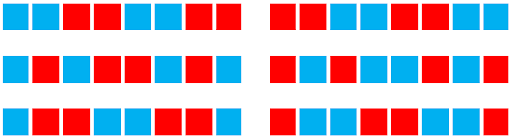
\includegraphics[width=0.95\linewidth]{van der waerden.png}
        \caption{Ejemplo de 2-coloración en $[9]$}
        \label{fig:placeholder}
    \end{figure}
\end{frame}

\begin{frame}{Teorema de Van der Waerden}
    \begin{block}{Teorema finito (Van der Waerden, 1927)}
        Para todo entero positivo $r$, $k$ existe un mínimo entero positivo $W(r,k)$ tal que toda $r$-coloración de $[n]=\{1,2,\dots,n\}$, con $n\geq W(r,k)$, contiene una progresión aritmética monocromática de tamaño $k$.
    \end{block}
    
    \begin{block}{Teorema infinito (Van der Waerden, 1927)}
        Toda coloración finita de $\mathbb{Z}^{+}$ contiene una progresión aritmética monocromática \textbf{arbitrariamente grande}.
    \end{block}

    \pause
    \begin{block}{Cota de números de Van der Waerden (Timothy Gowers, 2001)}
        $$W(r, k) \le 2^{2^{r^{2^{2^{k+9}}}}}$$
    \end{block}
\end{frame}


% 6. Densidad natural (1 min)
\section{Densidad Natural}
\begin{frame}{Densidad natural}
    \begin{block}{Definición}
        Sea $A\subseteq\mathbb{N}$ la \textit{densidad natural} de $A$ como $$d(A)=\limsup_{n\to\infty}{\frac{\left|A\cap\{1,2,\dots,n\}\right|}{n}}=\inf_{n\geq 0}\sup_{m\geq n}{\frac{\left|A\cap\{1,2,\dots,n\}\right|}{n}}$$
        Si $A$ es finito, entonces, $d(A)=0$.
    \end{block}

    \begin{center}
        \begin{align*}
        d(n\mathbb{N})=\frac{1}{n} \qquad
        d(\{n^{2}:n\in\mathbb{N}\})=0 \qquad
        d(\{p:p\text{ es primo}\}) = 0
        \end{align*}
    \end{center}
    
\end{frame}


% 7. Teorema de Szemerédi (4 min)
\section{Teorema de Szemerédi}
% DIAPOSITIVA 1: Contexto Histórico y Concepto Clave
\begin{frame}{Teorema de Szemerédi: Contexto Histórico}

    \begin{columns}

        \begin{column}{0.6\textwidth}
            Propuesto como conjetura por \textbf{Erdős y Turán} en
            1936, no fue hasta \textbf{1975} que \textbf{Endre
            Szemerédi} logró demostrarlo, obteniendo el
            \textbf{Premio Abel}.

            \vspace{0.4cm}

            \begin{block}{Concepto Clave: Densidad vs.\ Color}
                Mientras que Ramsey trabaja con \textit{coloraciones},
                Szemerédi trabaja con \textbf{densidad}: si un
                subconjunto de enteros es lo suficientemente
                ``grueso'', debe contener progresiones aritméticas.
            \end{block}
        \end{column}

        \begin{column}{0.4\textwidth}
            \begin{exampleblock}{Conexiones}
                \begin{itemize}
                    \item Teoría de números
                    \item Teoría ergódica
                    \item Informática (TCS)
                \end{itemize}
            \end{exampleblock}
        \end{column}

    \end{columns}

\end{frame}


% DIAPOSITIVA 2: Definición Formal
\begin{frame}{Teorema de Szemerédi: Enunciado Formal}

    \begin{alertblock}{Teorema (Szemerédi, 1975)}
        Sea $A \subseteq \{1, 2, \dots, N\}$. Para todo entero
        $k \geq 3$ y todo $\delta > 0$, existe $N(\delta, k)$ tal
        que si
        $$|A| \geq \delta N$$
        entonces $A$ contiene una \textbf{progresión aritmética de
        longitud $k$}.
    \end{alertblock}

    \pause
    \vspace{0.3cm}

    \begin{block}{Diferencia con Ramsey Tradicional}
        \begin{itemize}
            \item \textbf{Ramsey:} al dividir en $r$ colores, algún
                  color contendrá el patrón.
            \item \textbf{Szemerédi:} \textit{cualquier} conjunto con
                  densidad positiva contiene el patrón, sin necesidad
                  de considerar todas las clases.
        \end{itemize}
    \end{block}

\end{frame}


% DIAPOSITIVA 3: El Lema de Regularidad y Conclusión
\begin{frame}{El Lema de Regularidad de Szemerédi}

    Para demostrar el teorema, Szemerédi introdujo el
    \textbf{Lema de Regularidad}, hoy una herramienta fundamental
    en combinatoria:

    \begin{enumerate}
        \item \textbf{Partición en bloques:} Cualquier grafo grande
              puede dividirse en bloques más pequeños.
        \item \textbf{Comportamiento pseudo-aleatorio:} La mayoría de
              los bloques se comportan de manera casi aleatoria
              (``regular'').
        \item \textbf{Estructura forzada:} La regularidad hace
              inevitable la aparición de progresiones aritméticas.
    \end{enumerate}

    \pause
    \vspace{0.3cm}

    \begin{block}{Conclusión}
        El Teorema de Szemerédi refuerza la máxima de Ramsey:
        \textbf{la estructura es inevitable}. Si seleccionas una
        fracción constante de los enteros, no importa cuán caótica
        sea tu elección; terminarás creando una progresión aritmética
        perfecta, por \textit{pura necesidad matemática}.
    \end{block}

\end{frame}


% 8. Teorema de Green-Tao (5 min)
\section{Teorema de Green-Tao}
% ============================================================
% SECCIÓN 8 — Teorema de Green-Tao (5 min)
% ============================================================

% --- Diapositiva 1: El problema de densidad cero ---
\begin{frame}{Green-Tao: El Obstáculo}

    \begin{block}{Recordatorio — Szemerédi}
        Garantiza PA de cualquier longitud en conjuntos con
        $d(A) > 0$.
    \end{block}

    \vspace{0.3cm}

    Por el \textbf{Teorema de los Números Primos}:
    \[
        \pi(n) \sim \frac{n}{\ln n}
        \quad\Longrightarrow\quad
        d\bigl(\{p : p \text{ es primo}\}\bigr)
        = \lim_{n\to\infty}\frac{\pi(n)}{n} = 0
    \]

    \pause
    \vspace{0.3cm}

    \begin{alertblock}{Obstáculo}
        $d(\text{primos}) = 0 \;\Rightarrow\;$ \textbf{Szemerédi no aplica}.\\[4pt]
        ¿Contienen los primos progresiones aritméticas
        arbitrariamente largas?
    \end{alertblock}

    \pause
    \vspace{0.3cm}

    \begin{exampleblock}{Respuesta (Green y Tao, 2004)}
        \centering
        \textbf{¡Sí!} Los primos contienen PA de cualquier
        longitud finita $k$.
    \end{exampleblock}

\end{frame}


% --- Diapositiva 2: Ejemplos visuales ---
\begin{frame}{Ejemplos de PA en los Primos}

    \begin{columns}[T]

        \begin{column}{0.55\textwidth}
        \begin{tikzpicture}[scale=0.85]
            % Números compuestos
            \foreach \n/\xi/\yi in {
                1/0/0, 4/3/0, 6/5/0,
                8/1/1, 9/2/1, 10/3/1, 12/5/1,
                14/1/2, 15/2/2, 16/3/2, 18/5/2,
                20/1/3, 21/2/3, 22/3/3, 24/5/3,
                25/0/4, 26/1/4, 27/2/4, 28/3/4, 30/5/4}{
                \filldraw[gray!25, draw=gray!45]
                    ({0.85*\xi},{-0.85*\yi}) circle (0.37cm);
                \node[text=gray!60, font=\scriptsize]
                    at ({0.85*\xi},{-0.85*\yi}) {\n};
            }
            % Primos normales
            \foreach \n/\xi/\yi in {2/1/0, 3/2/0, 7/0/1, 13/0/2, 19/0/3}{
                \filldraw[orange!65, draw=orange!85!black]
                    ({0.85*\xi},{-0.85*\yi}) circle (0.37cm);
                \node[text=black, font=\scriptsize\bfseries]
                    at ({0.85*\xi},{-0.85*\yi}) {\n};
            }
            % PA: 5,11,17,23,29 con d=6
            \foreach \n/\xi/\yi in {5/4/0, 11/4/1, 17/4/2, 23/4/3, 29/4/4}{
                \filldraw[red!70, draw=red!90!black]
                    ({0.85*\xi},{-0.85*\yi}) circle (0.37cm);
                \node[text=white, font=\scriptsize\bfseries]
                    at ({0.85*\xi},{-0.85*\yi}) {\n};
            }
            % Caja PA
            \draw[red, very thick, rounded corners=4pt]
                ({0.85*4-0.44}, 0.44) rectangle
                ({0.85*4+0.44}, {-0.85*4-0.44});
            \node[red, font=\small\bfseries]
                at ({0.85*4}, {-0.85*4-0.82}) {$d=6$};
            % Leyenda
            \filldraw[gray!25,   draw=gray!45]         (5.5,-0.20) circle (0.18cm);
            \node[font=\tiny, right=1pt] at (5.72,-0.20) {Compuesto};
            \filldraw[orange!65, draw=orange!85!black] (5.5,-0.65) circle (0.18cm);
            \node[font=\tiny, right=1pt] at (5.72,-0.65) {Primo};
            \filldraw[red!70,    draw=red!90!black]    (5.5,-1.10) circle (0.18cm);
            \node[font=\tiny, right=1pt, red] at (5.72,-1.10) {Primo en PA};
        \end{tikzpicture}
        \end{column}

        \begin{column}{0.42\textwidth}
            \textbf{Ejemplos concretos:}
            \begin{align*}
                k=3\colon &\quad 3,\;7,\;11 \\[3pt]
                k=5\colon &\quad 5,\;11,\;17,\;23,\;29 \\[3pt]
                k=10\colon &\quad 199,\;\ldots,\;2089
            \end{align*}

            \vspace{0.3cm}

            \begin{block}{Cuadro comparativo}
            {\footnotesize
            \begin{tabular}{ll}
                \hline
                VdW     & coloración $\to$ PA \\
                Szem.   & $d>0$ $\to$ PA \\
                G-T     & primos ($d=0$) $\to$ PA \\
                \hline
            \end{tabular}}
            \end{block}
        \end{column}

    \end{columns}

\end{frame}


% --- Diapositiva 3: Idea de la demostración ---
\begin{frame}{Idea de la Demostración de Green-Tao}

    \begin{columns}[T]

        \begin{column}{0.5\textwidth}
            \begin{block}{El problema}
                Los primos tienen densidad $0$, por lo que
                Szemerédi no aplica directamente.
            \end{block}

            \vspace{0.3cm}

            \textbf{Idea clave:} encontrar un conjunto \textit{casi
            primo} $B$ con:
            \begin{enumerate}
                \item $d(B) > 0$ dentro de $B$, los primos son
                      ``densos''.
                \item Los primos se comportan \textbf{pseudo-aleatoriamente}
                      dentro de $B$.
            \end{enumerate}
        \end{column}

        \begin{column}{0.46\textwidth}
            \begin{exampleblock}{Ingredientes}
                \begin{itemize}
                    \item Criba de Goldston-Pintz-Yildirim
                    \item Generalización de Szemerédi a\\
                          entornos pseudo-aleatorios
                    \item Teoría ergódica y análisis\\
                          de Fourier
                \end{itemize}
            \end{exampleblock}

            \vspace{0.3cm}

            \begin{alertblock}{Impacto}
                Premio Salem 2004 (Green)\\
                Medalla Fields 2006 (Tao)
            \end{alertblock}
        \end{column}

    \end{columns}

\end{frame}


% 9. Conclusiones
% ============================================================
% SECCIÓN 9 — Conclusiones
% ============================================================

\section{Conclusiones}

% --- Diapositiva 1: La cadena de resultados ---
\begin{frame}{El Arco de la Teoría de Ramsey}

    \begin{center}
    \begin{tikzpicture}[
        node distance=0.6cm and 0.4cm,
        boxa/.style={draw, rounded corners=4pt, fill=blue!60,   text=white,
                     font=\small\bfseries, minimum width=2.4cm,
                     minimum height=0.7cm, align=center},
        boxb/.style={draw, rounded corners=4pt, fill=teal!65,   text=white,
                     font=\small\bfseries, minimum width=2.4cm,
                     minimum height=0.7cm, align=center},
        boxc/.style={draw, rounded corners=4pt, fill=violet!65, text=white,
                     font=\small\bfseries, minimum width=2.4cm,
                     minimum height=0.7cm, align=center},
        boxd/.style={draw, rounded corners=4pt, fill=orange!70, text=white,
                     font=\small\bfseries, minimum width=2.4cm,
                     minimum height=0.7cm, align=center},
        boxe/.style={draw, rounded corners=4pt, fill=red!65,    text=white,
                     font=\small\bfseries, minimum width=2.4cm,
                     minimum height=0.7cm, align=center},
        arr/.style={->, thick, gray!70}
    ]
        \node[boxa] (ramsey) {Teoría de\\Ramsey};
        \node[boxb, right=0.5cm of ramsey] (schur)  {Schur\\(1916)};
        \node[boxc, right=0.5cm of schur]  (vdw)    {Van der\\Waerden (1927)};
        \node[boxd, below=0.8cm of schur]  (szem)   {Szemerédi\\(1975)};
        \node[boxe, right=0.5cm of szem]   (gt)     {Green-Tao\\(2004)};

        \draw[arr] (ramsey) -- (schur);
        \draw[arr] (schur)  -- (vdw);
        \draw[arr] (vdw)    -- (szem);
        \draw[arr] (szem)   -- (gt);

        \node[font=\tiny, gray, below=0.15cm of ramsey] {patrones inevitables};
        \node[font=\tiny, gray, below=0.15cm of schur]  {$x{+}y{=}z$ mono.};
        \node[font=\tiny, gray, below=0.15cm of vdw]    {PA mono.};
        \node[font=\tiny, gray, below=0.15cm of szem]   {$d{>}0 \to$ PA};
        \node[font=\tiny, gray, below=0.15cm of gt]     {primos $\to$ PA};
    \end{tikzpicture}
    \end{center}

    \vspace{0.2cm}

    \begin{block}{El mensaje central}
        Cada resultado extiende el anterior, forzando más orden
        en contextos donde parecía no haberlo.
        \textbf{La estructura aritmética es inevitable.}
    \end{block}

\end{frame}


% --- Diapositiva 2: Reflexión final ---
\begin{frame}{Conclusiones}

    \begin{exampleblock}{\centering Principio de Motzkin — revisitado}
        \centering
        \Large\textit{``El desorden completo es imposible.''}
    \end{exampleblock}

    \vspace{0.35cm}

    \begin{columns}[T]
        \begin{column}{0.48\textwidth}
            \textbf{Lo que aprendimos:}
            \begin{itemize}
                \item El \textbf{Palomar} es el germen de todo.
                \item \textbf{Schur} y \textbf{VdW} garantizan
                      estructuras en coloraciones.
                \item \textbf{Szemerédi} solo necesita densidad positiva.
                \item \textbf{Green-Tao} vence incluso a la
                      densidad nula de los primos.
            \end{itemize}
        \end{column}
        \begin{column}{0.48\textwidth}
            \textbf{Preguntas abiertas:}
            \begin{itemize}
                \item ¿Cuánto vale $R(5,5)$?
                \item Cotas exactas de $W(r,k)$.
                \item ¿PA en los primos gemelos?
                \item Conjetura de Erdős sobre PA en
                      conjuntos de series divergentes.
            \end{itemize}
        \end{column}
    \end{columns}

    \pause
    \vspace{0.35cm}

    \begin{alertblock}{\centering Mensaje final}
        \centering
        En matemáticas, los \textbf{patrones no son casualidad}:
        son una consecuencia \textbf{inevitable} del tamaño.
    \end{alertblock}

\end{frame}


\end{document}
